\chapter{Curbe Eliptice} 
\section{Introducere}
\label{sec:sec01}
Folosirea curbelor eliptice in criptografie a fost propusa pentru prima oara in anul 1985 de Victor Miller(IBM) si, independent, de Neal Koblitz. Ideea de baza este folosirea grupului de puncte de pe o curba eliptica in locul grupului $(\mathbb{Z}/p\mathbb{Z})^{*}$. Printre aplicatiile practice ale curbelor eliptice se numara constructia criptosistemelor cu chei publice, construirea de generatoare pseudoaleatoare de biti, teoria codurilor, teste de primalitate, etc.
\begin{dfn}
[sursa Guide to elliptic curves menezez]O \textit{curba eliptica} $E$ peste un corp $K$ este definita prin ecuatia:
$$E : y^2 + a_1xy + a_3y = x^3 + a_2x^{2} + a_4x + a_6$$ 
\\unde $a_1, a_2, a_3, a_4, a_5, a_6\in K$, iar discriminantul ecuatiei, $\Delta \neq 0$. Discriminantul ecuatiei este definit astfel:
$$ \begin{cases}
\Delta = -d_2^{2}d_8 - 8d_4^{3} - 27d_6^{2} + 9d_2d_4d_6 \\
d_2 = a_1^{2} + 4a_2 \\
d_4 = 2a_4 + a_1a_3 \\
d_6 = a_3^{2} + 4a_6 \\
d_8 = a_1^{2}a_6 + 4a_2a_6 - a_1a_3a_4 + a_2a_3^{2} - a_4^{2}
\end{cases}$$
\end{dfn}
\begin{dfn}
Fie $L$ orice extensie a corpului $K$. Definim multimea de $L$-puncte rationale peste $E$ astfel: $E(L) = \set {(x, y)\in L\times L: y^2 + a_1xy + a_3y - x^3 - a_2x^{2} - a_4x - a_6 = 0} \cup \set {\infty}$
\end{dfn}
\begin{obs}
In urmatoarele randuri voi face o serie de observatii asupra ecuatiei unei curbe eliptice: \\
(i) Ecuatia de la definitia 2.1 se numeste Ecuatie Weierstrass \\
(ii) Conditia ca discriminantul $\Delta$ sa fie diferit de 0 asigura "netezimea" curbei eliptice, adica nu exista puncte care sa aibe 2 sau mai multe tangente diferite la curba. \\
(iii) L-punctele rationale sunt acele puncte, $(x, y)$ care satisfac ecuatia Weierstrass, cu $x, y \in L$. Punctul de la infinit este considerat un punct L-rational pentru toate extensiile $L$ ale corpului $K$
\end{obs}

\begin{dfn}
Fie $E_1, E_2$ doua curbe eliptice, definite astfel: \\
$E_1 : y^2 + a_1xy + a_3y = x^3 + a_2x^{2} + a_4x + a_6$ \\
$E_2 : y^2 + \overline{a_1}xy + \overline{a_3}y = x^3 + \overline{a_2}x^{2} + \overline{a_4}x + \overline{a_6} $ \\
Spunem ca cele doua curbe sunt \textit{izomorfe} daca exista $u,r,s,t\in K, u\neq 0$ astfel incat schimbarea de variabila $(x, y)\rightarrow (u^2x + r, u^3y + u^2sx + t)$ transforma ecuatia $E_1$ in ecuatia $E_2$. Acest tip de transformare se numeste schimbare "admisibila" de variabila.
\end{dfn}
\begin{dfn}
Ecuatia Weierstrass a unei curbe eliptice poate fi simplificata in mod considerabil, aplicand schimbari admisibile de variabila. Vom trata trei cazuri separate de schimbari de variabila, in functie de caracteristica corpului $K$, ajungand la o forma \textit{simplificata a Ecuatiei Weierstrass.}. Vom aborda trei cazuri, primul fiind $char(K) \neq \set {2,3}$ \\

  1. Fie $K$ un corp si \textit{E} o curba eliptica data prin ecuatia lui Weierstrass. O schimbare admisibila de variabila este:
$(x, y) \rightarrow (\frac{x - 3a_1^{2} - 12a_2}{36}, \frac{y-3a_1x}{216} - \frac{a_1^{3} + 4a_1a_2 - 12a_3}{24})$ \\
Aceasta schimbare transforma ecuatia $E$ in ecuatia 
\begin{center} $y^2 = x^3 + ax + b; a, b\in K$\end{center}
Discriminantul acestei noi ecuatii este $\Delta = -16(4a^3 + 27b^2)$ \\

2. Daca $char(K) = 2$ trebuie sa consideram doua subcazuri. Daca $a_1 \neq 0$, atunci o schimbare admisibila de variabila este: $(x, y) \rightarrow (a_1^2x + \frac{a_3}{a_1}, a_1^3y + \frac{a_1^2a_4 + a_3^2}{a_1^3} )$, care transforma $E$ in:
\begin{center}$y^2 + xy = x^3 + ax^2 + b; a, b\in K$\end{center}
O astfel de ecuatie se numeste \textit{non-supersingulara} si are discriminantul $\Delta = b$ \\
Daca $a_1 = 0$ atunci o schimbare admisibila ar fi $(x, y)\rightarrow (x + a_2, y)$ care transforma curba $E$ in
\begin{center} $y^2 + cy = x^3 + ax + b; a,b,c\in K$ \end{center}
O astfel de ecuatie se numeste \textit{supersingulara} si are discriminantul $\Delta = c^4$
\\

3. Daca $char(K) = 3$ trebuie sa consideram din nou doua subcazuri. Daca $a_1^2 \neq -a_2$ atunci o schimbare admisibila de variabila este
$(x, y) \rightarrow (x + \frac{\alpha}{\beta}, y + a_1x + a_1\frac{\alpha}{\beta} + a_3)$, unde $\alpha = a_4 -a_1a_3$ si $\beta = a_1^2 - a_2$. Ecuatia $E$ devine: 
\begin{center} $y^2 = x^3 + ax^2 + b; a, b\in K$\end{center}
O astfel de ecuatie se numeste \textit{non-supersingulara} si are discriminantul $\Delta = -a^3b$ \\
Daca $a_1^2 = -a_2$ atunci consideram o schimbare admisibila de variabila $(x, y) \rightarrow (x, y + a_1x + a_3)$ care transforma curba $E$ in:
\begin{center} $y^2 = x^3 + ax + b$ \end{center}
O astfel de curba este \textit{supersingulara} si are discriminantul $\Delta = -a^3$
\end{dfn}

\begin{obs}
Noi vom lucra cu forma simplificata a ecuatiei Weierstrass pe tot parcursul urmatoarelor capitole.
\end{obs}

\subsection{Constructia curbelor eliptice}
\label{subsec:subsec01}

\begin{dfn}
Fie $E$ o curba eliptica peste un corp $K = F_q$. Multimea de puncte $E(F_q)$ impreuna cu operatia de adunare formeaza o structura de grup abelian, cu punctul de la infinit fiind identitatea din grup. Acest grup este folosit in criptografia bazata pe curbe eliptice.
\end{dfn}

\begin{dfn}
Numim \textit{ordin} al unei curbe eliptice, numarul de puncte care satisfac ecuatia Weierstrass, cu alte cuvinte cardinalul multimii $E(F_q)$ si il notam cu $\# E(F_q)$. Teorema care urmeaza, datorata lui \textit{Hasse}, ofera o aproximare pentru acest ordin
\end{dfn}
\begin{teo}
Fie $E$ o curba eliptica definita peste $F_q$. Atunci este adevarata relatia:
\begin{center} $q + 1 - 2\sqrt{q}\leq \# E(F_q)\leq q+1 + 2\sqrt{q}$ \end{center}
Intrucat $2\sqrt{q}$ este relativ mic in comparatie cu $q$, putem afirma ca $\# E(F_q) \approx q$
\end{teo}
\begin{teo}
Fie $q = p^m$, unde $p$ este caracteristica corpului $F_q$. Atunci exista o curba eliptica $E$ definita peste acest corp, cu $\# E(F_q) = q+1-t$ ($t$ se numeste urma curbei eliptice $E$) daca si numai daca una dintre urmatoarele conditii este adevarata: \\
(i) $t \not\equiv 0$ mod $p$ si $t^2\leq 4q$ \\
(ii) m este impar si $t=0$ sau $t^2 = 2q$ si $p=2$ sau $t^2 = 3q$ si $p=3$ \\ 
(iii) m este par si $t^2 = 4q$ sau $t^2 = q$ si $p\not\equiv 1$ mod $3$ sau $t= 0$ si $p\not\equiv 1$ mod $4$
\end{teo}
\begin{dfn}
Fie $p$ caracteristica corpului $F_q$. Numim curba eliptica \textit{supersingulara}, daca $p$ divide $t$, unde t este urma curbei. Altfel, curba $E$ este \textit{non-supersingulara}
\end{dfn}
\begin{teo}
Fie $E$ o curba eliptica peste corpul $F_q$ si fie ordinul acesteia $\# E(F_q)= q+ 1-t$. Atunci, $\# E(F_q) = q+ 1 - V_n$, unde definim sirul $\set {V_n}$ recursiv prin formula $V_0 = 2, V_1=t$ si $V_n = V_1V_{n-1} - qV_{n-2}, \forall n\geq 2$
\end{teo}
Urmatoarea teorema descrie structura grupului pentru o curba eliptica. Vom nota un grup ciclic de ordin n, cu $Z_n$.
\begin{teo}
Fie E o curba eliptica definita peste $F_q$. Atunci $E(F_q)$ este izomorfic cu $Z_{n_1} \oplus Z_{n_2}$, unde $n_1, n_2\in Z$, unici determinati, cu $n_2$ care divide atat $n_1$ cat si $q-1$. Daca $n_2=1$, spunem ca $E(F_q)$ este grup ciclic.
\end{teo}

\subsection{Reprezentari ale punctelor de pe o curba eliptica}
\label{subsec:subsec02}
De multe ori, in efectuarea operatiile pe curbe eliptice, poate fi avantajos sa reprezentam un punct in alte coordonate decat cele afine(sectiunea 2.3.1). De exemplu, in calculul sumei a doua puncte(operatie care la randul ei este folosita in algoritmii pentru inmultirea cu un scalar si in inmultirea multipla) se observa necesitatea de a efectua operatia de invers modular de mai multe ori. Acesta operatie este costisitoare din punct de vedere computational, astfel vom folosi diferite tipuri de reprezentari.
\begin{dfn}
Fie $K$ un corp si $c, d\in \mathbb{N}$. Definim o relatie de echivalenta peste multimea $K^3\setminus \set {(0, 0, 0)}$ ca fiind :
\begin{center} $(X_1, Y_1, Z_1) \equiv (X_2, Y_2, Z_2)$ daca $X_1 = \lambda ^cX_2, Y_1 = \lambda ^d Y_2, Z_1 = \lambda Z_2, \lambda\in K^{*}$\end{center}
Exista o corespondenta $1-1$ intre multimea de puncte in coordonate proiective $P(K)^{*} = \set {(X, Y, Z): X, Y, Z\in K, Z\neq 0}$ si multimea punctelor in coordonate afine, $A(K) = \set {(x, y): x, y\in K}$
\end{dfn}
\begin{dfn}
Consideram $c=1, d=1$ in definitia \textit{coordonatelor proiective}. Acestea se numesc \textit{coordonate proiective standard}. Punctu l in coordonate proiective $(X, Y, Z), Z\neq 0$ corespunde punctului in coordonate afine $(X/Z, Y/Z)$. Ecuatia curbei eliptice devine:
\begin{center}  $Y^2Z = X^3 + aXZ^2 + bZ^3$ \end{center}
Punctul de la infinit este $(0, 1, 0)$ in timp ce inversul unui punct oarecare este $(X, -Y, Z)$
\end{dfn}
\begin{dfn}
Consideram $c=2, d=3$. Acest sistem de coordonate se numesc coordonate \textit{proiective Jacobi}. Punctul $(X, Y, Z), Z\neq 0$ corespunde punctului 
in coordonate afine $(X/Z^2, Y/Z^3)$. Ecuatia curbei devine:
\begin{center} $Y^2 = X^3 + aXZ^4 + bZ^6$ \end{center}
Punctul de la infinit este $(1, 1, 0)$, iar inversul unui punct este $(X, -Y, Z)$
\end{dfn}
\begin{dfn}
\textit{Coordonatele Chudnovsky} sunt obtinute din coordonatele Jacobi, adaugand niste reduntante. Astfel, un punct reprezentat in acest tip de coordonate, arata in acest fel : $(X, Y, Z, Z^2, Z^3)$. Acest tip de reprezentare aduce imbunatatiri de performanta cand folosim anumiti algoritmi specializati pentru inmultirea cu un scalar.
\end{dfn}

\begin{obs}
Se poate folosi $Z = 1$ in implementari pentru a simplifica calculele.
\end{obs}

\section{Aritmetica curbelor eliptice}
\label{sec:sec02}
In aceasta sectiune vom prezenta operatiile din corpul finit format de punctele de pe o curba eliptica(adunarea,  inmultirea cu un scalar) precum si operatia de inmultire multipla cu scalari. La inceput vom oferi o privire de ansamblu asupra acestor operatii, oferind definitii, apoi vom intra in delalii in sectiunea 2.3, oferind inclusiv implementarea unor algoritmi eficienti pentru aceste operatii.

\begin{dfn}
Adunarea a doua puncte de pe o curba eliptica este foarte intuitiva din punct de vedere geometric. Fie $P, Q$ doua puncte si $R$ suma lor. Rezultatul este obtinut astfel. Mai intai desenam o linie intre $P, Q$. Acesta linie intersecteaza curba intr-ul al treilea punct. Punctul $R$ este reflectia la axa $Ox$ a acestui punct(Figura 2.1a). Dublul unui punct $P(2P = R)$ este definit astfel. Desenam o tangenta la curba eliptica in P, aceasta intersectand curba intr-un punct secundar. Punctul $R$ este din nou reflexia la axa $Ox$(Figura 2.1b).  
\end{dfn}

\begin{obs}
Formulele algebrice pentru adunarea a doua puncte difera in functie de sistemul de coordnate folosit, sau tipul de corp algebric peste care este definita curba eliptica(corp prim, binar sau de extensie).
\end{obs}

\begin{figure}[htp]
\centering
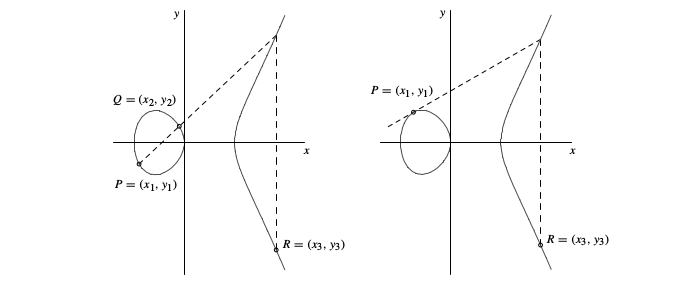
\includegraphics[width=13cm]{chapters/Addition.png}
\caption{Adunarea si dublarea unui punct pe o curba eliptica}
\label{fig:lion}
\end{figure}

\begin{dfn}
O alta operatie fundamentala este cea a inmultirii unui punct $P$ de pe o curba eliptica, cu un scalar, $k\in \mathbb{Z}$. Exista multe metode de a face acest lucru, de la metoda brute force de a face k adunari repetate pana la metode mai rafinate, precum cea a ferestrei glisante, care inbunatatesc considerabil performanta operatiei. Vom discuta in sectiunile care urmeaza algoritmi eficienti de inmultire. 
\end{dfn}

\begin{dfn}
O operatie asemanatoare celei de inmultire cu un scalar, este cea de inmultire multipla cu scalari. Fie doua puncte, $P, Q$ de pe o curba eliptica si doi scalari, $k, l\in \mathbb{Z}$. Dorim sa aflam rezultatul $kP + lQ$. Evident, precum la operatia de inmultire cu un scalar putem aplica o metoda directa, de a inmulti punctul $P$ cu scalarul $k$ respectiv punctul $Q$ cu scalarul $l$ si apoi facem o adunare de puncte. Acest lucru este insa ineficient, intrucat exista si aici metode mai rapide de a calcula acest lucru. Aceasta operatie de inmultire rapida este una extrem de folosita in criptografia pe curbe eliptice, aparand de exemplu, in cadrul unor protocoale criptografice, precum ECDSA, iar implementarea ineficienta e acesteia duce la mari probleme de performanta. 
\end{dfn}

\begin{obs}
Operatia de adunare pe o curba eliptica este corespondenta operatiei de inmultire
in sistemele cu chei publice obisnuite, iar adunarea multipla este corespondenta
exponentierii modulare din acestea.
Desi regulile de calcul in grupul punctelor unei curbe eliptice par destul de complicate, aritmetica acestora poate fi implementata extrem de eflcient, calculele in acest grup fiind realizate mult mai rapid decat cele din grupul $Z_p$, deoarece operatia de invers este una necostisitoare din punct de vedere computational.
\end{obs}

\section{Studiu Comparativ}
\label{sec:sec03}
In aceasta subsectiune voi aborda cele trei operatii de baza, adunarea, inmultirea cu un scalar si inmultirea multipla, prezentand la fiecare sectiune o analiza a eficientei metodei alese. Implementarea eficienta si corecta a acestor operatii reprezinta un prim pas foarte important spre dezvoltarea unor criptosisteme bazate pe curbe eliptice.
\\ Pentru implementare am ales limbajul de programare Python, versiunea 3.5.2, iar hardware-ul folosit in tabelele de test este: Quad Core CPU, i7-4700HQ, 2.4 GHz, 64 bit OS, 16 GB RAM.

\subsubsection{Arhitectura aplicatiei}
\label{sec:sec01}
arhitectura(Inclusiv grupul folosit, curbele eliptice Nist), diagrama UML cu clasele

\subsection{Metode de adunarea a punctelor de pe o curba eliptica, comparatie}
\label{subsec:subsec02}
In aplicatie am implementat operatia de adunare pentru coordonate Afine si pentru coordonate Jacobiene. Vom oferi formulele de calcul pentru cele tipuri de adunare si apoi vom compara eficienta celor doua implementari.
\begin{dfn}
Pentru puncte reprezentate prin coordonate afine formulele de calcul sunt dupa cum urmeaza.Fie 2 puncte, $P(x_{1}, y_1), Q(x_2, y_2)\in E(F_p)$. Notam cu $R(x_3, y_3) = P + Q$. Formulele pentru adunarea a doua puncte pot fi demonstrate matematic destul de usor, pornind de la ideea ca $P, Q$ si reflexia rezultatului la axa $Ox$ se afla pe aceasi dreapta, respectiv pe aceasi curba eliptica.

$\begin{cases} 
    x_3 = \lambda^2 - x_1 - x_2 \\
    y_3 =  \lambda (x_1-x_3) - y_1
   \end{cases}$
 \\cu 
 \\$
 \lambda = 
 \begin{cases}
 \frac{y_2 - y_1}{x_2 - x_1}, P \neq Q \\ 
 \frac{3x^{2}_1 + a}{2y_1}, P = Q
 \end{cases}$ \\
\end{dfn}

\begin{dem}
Fie $P(x_1, y_1), Q(x_2, y_2)\in E(F_p)$ Punctele se afla pe aceasi dreapta. Scriind ecuatia dreptei care trece prin cele doua puncte si considerand ca $-R\in E(F_p)$, rezolvam sistemul de ecuatii:
$\begin{cases} 
    0 = \begin{vmatrix}
			x_1 & y_1 & 1 \\ 
			x_2 & y_2 & 1 \\ 
			x & y & 1  \\ 
			\end{vmatrix} \\
    y^2 =  x^3 + ax + b
   \end{cases}$
   Panta dreptei este $\lambda = \begin{cases}
 \frac{y_2 - y_1}{x_2 - x_1}, P \neq Q \\ 
 \frac{3x^{2}_1 + a}{2y_1}, P = Q
 \end{cases}$
 \\Inlocuind in formula curbei eliptice obtinem formulele din definita precedenta.
\end{dem}

Urmeaza sa explic algoritmii si o scurta interpretare a rezultatelor. Pot pune bucati de cod aici?

\begin{tabular}{ |p{3cm}||p{3cm}|p{3cm}|p{3cm}|  }
 \hline
 \multicolumn{4}{|c|}{Adunarea punctelor de pe curbe eliptice} \\
 \hline
 Curba NIST& Coordonate &Metoda &Timp de executie(secunde)\\
 \hline
 P192   & Afine    &Adunare& 5.22\\
 P192&Afine  & Dublare & 5.19\\
 P192 &Jacobiene & Adunare& 2.6\\
 P192&Jacobiene & Dublare & 2.61\\
 P224& Afine & Adunare & 6.66\\
 P224& Jacobiene & Adunare   &3.32\\
 P256& Afine  & Adunare& 8.47\\
 P256& Jacobiene  & Adunare& 4.52\\
 P384& Afine  & Adunare& 18.06\\
 P384& Jacobiene  & Adunare& 8.96\\
 \hline
\end{tabular}

\subsection{Inmultirea cu un scalar, comparatie}
\label{subsec:subsec03}
--> urmeaza explicatii algoritmi + interpretare. Scalarii au fost alesi random, 1000 de iteratii.

\begin{tabular}{ |p{5cm}||p{3cm}|p{3cm}|p{2cm}|p{1cm}|  }
 \hline
 \multicolumn{5}{|c|}{Curba P192} \\
 \hline
 Algortitm& Coordonate &Intervalul &Fereastra &Timp\\
 \hline
 Alg Binar & Afine  &$[2^{5},2^{32}]$& - & 2.48\\
 Alg Binar&Jacobiene  & $[2^{5},2^{32}]$ & - & 0.6\\
 Alg Binar&Jacobiene  & $[2^{128},2^{192}]$ & - & 3.88\\
 Inmultire de st. la dr. & Jacobian & $[2^{5},2^{32}]$& - & 0.39\\
 Inmultire de st. la dr. & Afine & $[2^{128},2^{192}]$& - & 14.04\\
 Inmultire de st. la dr. & Jacobian & $[2^{128},2^{192}]$& - & 2.49\\
 Inmultire de dr. la st. &Afine & $[2^{128},2^{192}]$ & - & 14.33\\
 Inmultire de dr. la st. &Jacobiene & $[2^{5},2^{32}]$ & - & 0.41\\
 Inmultire de dr. la st. &Jacobiene & $[2^{128},2^{192}]$ & - & 2.52\\
 Metoda cu fereastra& Jacobiene & $[2^{5},2^{32}]$ & 3 & 0.42\\
 Metoda cu fereastra& Jacobiene & $[2^{128},2^{192}]$ & 3 & 2.38\\
 Metoda cu fereastra& Jacobiene & $[2^{128},2^{192}]$ & 4 & 2.32\\
 Fereastra glisanta st. la dr.& Jacobiene  & $[2^{5},2^{32}]$& 3 & 0.51\\
 Fereastra glisanta st. la dr.& Jacobiene  & $[2^{128},2^{192}]$& 3 & 2.68\\
  Fereastra glisanta st. la dr.& Jacobiene  & $[2^{128},2^{192}]$& 4 & 2.04\\
 Fereastra glisanta dr. la st.& Jacobiene  & $[2^{128},2^{192}]$& 3 & 2.47\\
 Fereastra glisanta dr. la st.& Jacobiene  & $[2^{128},2^{192}]$& 4 & 2.41\\
 Fereastra glisanta dr. la st.& Jacobiene  & $[2^{128},2^{192}]$& 5 & 2.58\\
 \hline
\end{tabular}

\begin{tabular}{ |p{5cm}||p{3cm}|p{3cm}|p{2cm}|p{1cm}|  }
 \hline
 \multicolumn{5}{|c|}{Curba P384} \\
 \hline
 Algortitm& Coordonate &Intervalul &Fereastra &Timp\\
 \hline
 Alg Binar & Afine  &$[2^{5},2^{32}]$& - & 5.5\\
 Alg Binar&Jacobiene  & $[2^{5},2^{32}]$ & - & 1.12\\
 Alg Binar&Jacobiene  & $[2^{300},2^{384}]$ & - & 13.98\\
 Inmultire de st. la dr. & Jacobian & $[2^{5},2^{32}]$& - & 0.66\\
 Inmultire de st. la dr. & Afine & $[2^{300},2^{384}]$& - & 59.62\\
 Inmultire de st. la dr. & Jacobian & $[2^{128},2^{192}]$& - & 8.33\\
 Inmultire de dr. la st. &Afine & $[2^{300},2^{384}]$ & - & 59.58\\
 Inmultire de dr. la st. &Jacobiene & $[2^{5},2^{32}]$ & - & 0.69\\
 Inmultire de dr. la st. &Jacobiene & $[2^{300},2^{384}]$ & - & 8.69\\
 Metoda cu fereastra& Jacobiene & $[2^{5},2^{32}]$ & 3 & 0.68\\
 Metoda cu fereastra& Jacobiene & $[2^{300},2^{384}]$ & 3 & 8.2\\
 Metoda cu fereastra& Jacobiene & $[2^{300},2^{384}]$ & 4 & 7.89\\
 Fereastra glisanta st. la dr.& Jacobiene  & $[2^{5},2^{32}]$& 3 & 0.85\\
 Fereastra glisanta st. la dr.& Jacobiene  & $[2^{300},2^{384}]$& 3 & 8.73\\
  Fereastra glisanta st. la dr.& Jacobiene  & $[2^{300},2^{384}]$& 4 & 6.46\\
 Fereastra glisanta dr. la st.& Jacobiene  & $[2^{300},2^{384}]$& 3 & 8.17\\
 Fereastra glisanta dr. la st.& Jacobiene  & $[2^{300},2^{384}]$& 4 & 7.93\\
 Fereastra glisanta dr. la st.& Jacobiene  & $[2^{300},2^{384}]$& 5 & 8.33\\
 \hline
\end{tabular}	

\subsection{Inmultirea multipla, comparatie}
\label{subsec:subsec04}
Nu am obtinut rezultate bune la Interleaving.. Ar trebui sa aleg altfel ferestrele, sau e pur si simplu o problema la implementare? Scalarii au fost alesi random in intervalul specificat, 1000 de iteratii.

\begin{tabular}{ |p{5cm}||p{3cm}|p{3cm}|p{2cm}|p{1cm}|  }
 \hline
 \multicolumn{5}{|c|}{Curba P192} \\
 \hline
  Algortitm& Coordonate &Intervalul &Ferestre &Timp\\
 \hline
 Alg Brut & Afine  &$[2^{5},2^{32}]$& - & 4.85\\
 Alg Brut & Afine  &$[2^{128},2^{198}]$& - & 26.18 \\
 Alg Brut & Jacobiene  &$[2^{5},2^{32}]$& - & 1.04 \\
 Alg Brut & Jacobiene  &$[2^{128},2^{198}]$& - & 4.89 \\
 Inmultire cu JSF & Afine  &$[2^{5},2^{32}]$& - & 2.72 \\
 Inmultire cu JSF & Jacobiene  &$[2^{5},2^{32}]$& - & 0.56 \\
 Inmultire cu JSF & Jacobiene  &$[2^{128},2^{198}]$& - & 2.35 \\
 Interleaving & Jacobiene  &$[2^{5},2^{32}]$& 3, 4 & 0.66 \\
 Interleaving & Jacobiene  &$[2^{128},2^{198}]$& 3, 3 & 3.39\\
 Interleaving & Jacobiene  &$[2^{128},2^{198}]$& 3, 4 &  3.29\\
 Interleaving & Jacobiene  &$[2^{128},2^{198}]$& 4, 4 & 3.15 \\
 Interleaving & Jacobiene  &$[2^{128},2^{198}]$& 4, 5 & 3.4 \\
 Interleaving & Jacobiene  &$[2^{128},2^{198}]$& 5, 5 & 3.55 \\
 \hline
\end{tabular}

\begin{tabular}{ |p{5cm}||p{3cm}|p{3cm}|p{2cm}|p{1cm}|  }
 \hline
 \multicolumn{5}{|c|}{Curba P384} \\
  \hline
  Algortitm& Coordonate &Intervalul &Ferestre &Timp\\
 \hline
 Alg Brut & Afine  &$[2^{5},2^{32}]$& - & 10.81\\
 Alg Brut & Afine  &$[2^{128},2^{198}]$& - & 54.17 \\
 Alg Brut & Jacobiene  &$[2^{5},2^{32}]$& - & 1.69 \\
 Alg Brut & Jacobiene  &$[2^{128},2^{198}]$& - & 8.25 \\
 Inmultire cu JSF & Afine  &$[2^{5},2^{32}]$& - & 5.92 \\
 Inmultire cu JSF & Jacobiene  &$[2^{5},2^{32}]$& - & 0.9 \\
 Inmultire cu JSF & Jacobiene  &$[2^{128},2^{198}]$& - & 3.84\\
 Interleaving & Jacobiene  &$[2^{5},2^{32}]$& 3, 4 & 1.09 \\
 Interleaving & Jacobiene  &$[2^{128},2^{198}]$& 3, 3 & 5.31 \\
 Interleaving & Jacobiene  &$[2^{128},2^{198}]$& 3, 4 & 5.41 \\
 Interleaving & Jacobiene  &$[2^{128},2^{198}]$& 4, 4 & 5.23 \\
 Interleaving & Jacobiene  &$[2^{128},2^{198}]$& 4, 5 & 5.61 \\
 Interleaving & Jacobiene  &$[2^{128},2^{198}]$& 5, 5 & 5.83	 \\
 \hline
\end{tabular}



